\documentclass[]{resume-openfont}

\hypersetup{
pdftitle={SajadEbrahimi - CV},
pdfsubject={SajadEbrahimi - CV},
pdfauthor={Sajad Ebrahimi},
}

\resetHeaderAndFooter

%--------------------------------------------------------------
% Convenience command - make it easy to fill template

\newcommand{\resumeHeading}[4]{\runsubsection{#1}{, #2}\hfill\location{#3 | #4}\fakeNewLine}

\newcommand{\resumeHeadingWoLoc}[3]{\runsubsection{#1}{, #2}\hfill\location{#3}\fakeNewLine}


\newcommand{\publicationHeading}[3]{{#1}\hfill\location{#3}\\ \descript{#2}\\}


\newcommand{\projectHeading}[2]{\normalsize{\customLink{#2}{#1}}\\}

\newcommand{\publicationHeadingInline}[2]{%
  \begin{tabularx}{\linewidth}{@{}>{\centering\arraybackslash}p{1.25cm} X@{}}%
    \location{#2} & \descript{#1}%
  \end{tabularx}%
  \vspace{-2pt}%
}

 
%--------------------------------------------------------------
\begin{document}


%--------------------------------------------------------------
%     Profile
%--------------------------------------------------------------
\newcommand{\yourName}{Sajad Ebrahimi}
% How you want it to show up on the resume
\newcommand{\yourWebsite}{Homepage}
% vs how you want it to show up. If it's the same you can just replace "\yourWebsiteLink" with "yourWebsite"
\newcommand{\yourWebsiteLink}{https://sadjadeb.github.io/}
\newcommand{\yourEmail}{sadjadeb@gmail.com}
\newcommand{\yourPhone}{+14378184048}
\newcommand{\githubUserName}{sadjadeb}
\newcommand{\linkedInUserName}{sadjadeb}
\newcommand{\Twitter}{sadjadeb}
\newcommand{\yourGoogleScholar}{M03zdaAAAAAJ}
\newcommand{\yourLocation}{Toronto, ON}

\begin{center}
    % \Huge \scshape {\yourName} \\ \vspace{4pt}
    \fontsize{30 pt}{30 pt} {\color{headingtext}\textbf{\yourName}} \\ \vspace{4pt}
    \small 
    \customLink{mailto:\yourEmail}{\faEnvelope \: \yourEmail}
    $|$  \customLink{\yourWebsiteLink}{\faGlobe \: sadjadeb.github.io}
    $|$ \customLink{https://github.com/\githubUserName}{\faGithub \: \githubUserName}
    $|$ \customLink{https://www.linkedin.com/in/\linkedInUserName}{\faLinkedin \: LinkedIn}
    $|$  \customLink{https://scholar.google.co.in/citations?user=M03zdaAAAAAJ&hl=en\yourGoogleScholar}{\faGraduationCap \: Google Scholar}
    $|$ \faHome \: \yourLocation \\
\end{center}

% \begin{tikzpicture}[remember picture, overlay]
%     \node[anchor=north east, xshift=-0.5cm, yshift=-0.8cm] at (current page.north east)
%         {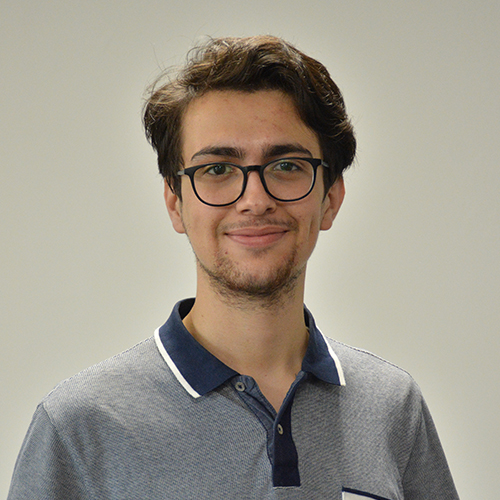
\includegraphics[width=2cm, height=2cm, keepaspectratio]{profile_pic.jpg}};
% \end{tikzpicture}

%--------------------------------------------------------------
%     Summary
%--------------------------------------------------------------
% \vspace{10pt}
\hspace{-21pt}
\section{Summary}
\vspace{-30pt}

\begin{bullets}[leftmargin=*]
    \item Graduate researcher in \textbf{\color{bodytext}NLP and Information Retrieval} with 20+ peer-reviewed publications (EMNLP, SIGIR, WSDM); focus on AI-Generated Content Detection, RAG Efficiency, Query Reformulation, and Peer Review Quality Assesment. 
    % For the latest list of my publications, please refer to \customLink{https://scholar.google.co.in/citations?user=M03zdaAAAAAJ&hl=en}{my Google Scholar}.
    
    \item Over 6 years of hands-on coding experience, spanning roles as a Data Scientist and a Software Engineer, specializing in designing, building, and deploying production-scale software and machine learning systems. Advanced proficiency in PyTorch, Django, Transformers, etc., with extensive experience delivering production-grade machine learning solutions.
\end{bullets}

\sectionsep

%--------------------------------------------------------------
%     Research Interests
%--------------------------------------------------------------
% \vspace{10pt}
% \hspace{-21pt}
% \section{Research Interests}
% \vspace{-10pt}
% \begin{multicols}{3}
%     \begin{bullets}
%         \item Natural Language Processing
%         \item Information Retrieval
%         % \item Data Mining
%         \item Diffusion Models
%     \end{bullets}
% \end{multicols}

% \vspace{-18pt}

% \begin{multicols}{3}
%     \begin{bullets}
%         \item Generative Ranking
%         \item Query Performance Prediction
%         \item Reviewer Assignment Problem
%     \end{bullets}
% \end{multicols}
% \vspace{-6pt}

%--------------------------------------------------------------
%     Education
%--------------------------------------------------------------
\section{Education}

% Put school first and degree second if your school is reputable

\resumeHeading{Ph.D. in Information}{University of Toronto}{Toronto, Canada}{Winter 2027 - }Supervisor: Dr. Ebrahim Bagheri \newline \\
\sectionsep

\resumeHeading{M.A.Sc. in Computer Engineering}{University of Guelph}{Guelph, Canada}{2023 - 2025}Supervisor: Dr. Fattane Zarrinkalam \enspace|\enspace Research Mentor: Dr. Bhaskar Mitra
\newline \\
Affiliated with \customLink{https://vectorinstitute.ai/}{Vector Institute for Artificial Intelligence} as Faculty Affiliate Researcher
\begin{bullets}
    % \item \textbf{GPA}: 89/100 
    % \item \textbf{Selected courses}: Information Retrieval(A+)
    \item \textbf{Thesis}: DiffusionRank: A Denoising Diffusion Framework for Learning to Rank
\end{bullets}
\vspace{4pt}
\sectionsep

\resumeHeading{B.Sc. in Computer Engineering}{Ferdowsi University of Mashhad}{Mashhad, Iran}{2018 - 2023}
% \begin{bullets}
    % \item \textbf{GPA}: 81/100
    % \item \textbf{Selected courses}: Fundamentals of Information Retrieval(A+), Data Mining(A+), Database(A+)
    % \item \textbf{Project}: Building Comprehensive Course Datasets from University Catalogs
% \end{bullets}
\sectionsep


% \educationHeading{High School Diploma in Mathematics}{\customLink{http://www.besat-hs.ir/}{Besat High School}}{Mashhad, Iran}{2014-2018}
% \begin{bullets}
%     \item \textbf{Overall GPA}: 4/4
% \end{bullets}
% \sectionsep


%--------------------------------------------------------------
%     Research Experience
%--------------------------------------------------------------
% \section{Internships and Research Experience}
\section{Research Experience}

\resumeHeadingWoLoc{Research Assistant}{University of Toronto}{Fall 2025 - Fall 2026}
Supervisor: Dr. Ebrahim Bagheri
\newline
\begin{bullets}
    \item Working on Retrieval-Augmented Generation (RAG) efficiency, Deep Research systems, and AI Generated Content Detection. 
\end{bullets}
\sectionsep


\resumeHeadingWoLoc{Graduate Research Assistant}{University of Guelph}{Fall 2023 - Summer 2025}

Supervisors: Dr. Fattane Zarrinkalam, Dr. Ebrahim Bagheri, and Dr. Bhaskar Mitra
\begin{bullets}
    \item Worked on applying the idea of DDPMs to Learning-to-Rank.
\end{bullets}
\sectionsep

\resumeHeadingWoLoc{Research Intern}{Toronto Metropolitan University}{Fall 2022 - Summer 2023}
Supervisor: Dr. Ebrahim Bagheri
\newline
\begin{bullets}
    \item Worked on Query Performance Prediction (QPP) and Enhancing retrievers by utilizing Entity Linking.
\end{bullets}
\sectionsep

\resumeHeadingWoLoc{Undergraduate Research Assistant}{Ferdowsi University of Mashhad}{Summer 2021 - Summer 2022}
Supervisor: Dr. Behshid Behkamal
\newline
\begin{bullets}
    % \item Created a structured dataset by designing a data format with 19 key course features and developing a scraper to collect course information from top-ranked universities' catalogs.
    \item Engineered datasets and automated data pipelines using schemas and scrapers for global university catalogs.
\end{bullets}
\sectionsep

%--------------------------------------------------------------
%     Work Experience
%--------------------------------------------------------------
\section{Work Experience}

\resumeHeading{Data Scientist}{\customLink{https://reviewer.ly/}{Reviewerly}}{Toronto, Canada}{Nov 2023 - }
\begin{bullets}
    \item Directed research on evaluating scientific peer reviews by defining 13 distinct metrics to assess review quality, resulting in the RottenReviews benchmark and Peeriscope tool.
    \item Built and now maintain a Milvus-backed index of 260M+ papers and 96M+ authors, delivering sub-second similarity search that powers Reviewerly's matching engine, adopted by peer-review venues and grant agencies in its first release cycle.
    % \item Designed and implemented an end-to-end pipeline to generate a made-to-order reviewer pool for each venue and assign appropriate reviewers to submissions.
    % \item Parallelized a keyphrase extraction model across 6 GPUs to process 200M records, accelerating the process by 10x.
\end{bullets}
\sectionsep


\resumeHeading{Data Analyst}{Kava Investment Analysis}{Tehran, Iran}{Sept 2021 - Aug 2022}
\begin{bullets}
    \item Built a scalable web scraper that collected data from 4+ sources across the Tehran Stock Exchange, reducing manual data collection time by 90\%.
    % \item Designed and implemented a PostgreSQL data warehouse: defined tables, indexes, and ETL pipelines for equities, bonds, and derivatives, which reduced query latency by 80\%.    
\end{bullets}
\sectionsep


% \resumeHeading{Software Engineer}{Freelance}{Iran}{March 2021 - April 2022}
% \begin{bullets}
%     \item Created the backend for the Bahar Charity website using Django Rest Framework. Users are enabled to settle appointment bills, while administrators can access diverse reports concerning invoices and appointments.
%     \item Engineered the Somchin mobile app employing Django Rest Framework. It facilitates the logging of cattle injuries and generates comprehensive reports throughout each treatment phase.
%     \item Devised a script for synchronizing databases across various grocery stores to streamline inventory tracking on an integrated platform.
% \end{bullets}
% \sectionsep


% \resumeHeading{Data Analyst Intern}{\customLink{https://almasdata.com/}{Almas Data}}{Mashhad, Iran}{July 2021 – Aug 2021}
% \begin{bullets}
%     \item Developed a script to crawl course data from various universities' course catalogs.
%     \item Preprocessed and cleaned data for machine learning training.
% \end{bullets}
% \sectionsep

\resumeHeading{Software Engineer Intern}{Zima \& Iliasystem Co.}{Mashhad, Iran}{Aug 2019 - Feb 2021}
\begin{bullets}
    % \item Acquired essential knowledge in backend development, REST API implementation, and database design by contributing to 3 internal tools and APIs used by a team of 10+ developers.
    \item Implemented REST APIs and DB schemas for 3 internal tools used by 10+ engineers; shipped 2 internal UIs (HTML/CSS/JS).
\end{bullets}
\sectionsep



%--------------------------------------------------------------
%     Skills
%--------------------------------------------------------------
\section{Skills}

% \bulletheader{Proficient in}: Machine Learning Algorithms, Neural Networks, Semantic Web, Information Retrieval
\bulletheader{Languages:}\  Python, C, C++ \\

\vspace{5pt}
% \bulletheader{Python Frameworks and Packages:}
%     \begin{bullets}
%         \item Accelerate, DeepSpeed, PyTorch, TensorFlow, Transformers, Pandas, NumPy, SKlearn, NLTK, spaCy, Beir
%         \item Django, Django Rest Framework, Flask, Fastapi
%         % \item Selenium, Pytest, Doctest, BeatifulSoup4
%         % \item python-telegram-bot, Tweepy
%     \end{bullets}
% \vspace{5pt}
\bulletheader{Databases:}\  PostgreSQL, MongoDB, SQLite, MySQL, Milvus \\
\vspace{5pt}
\bulletheader{Misc:}\  Git, Docker, Nginx, HTML/CSS, \LaTeX, Unix-based OS, REST API design, Web Scraping, Data Visualization \\
% \vspace{5pt}
% \bulletheader{Soft Skills:} Communication, Leadership, Teamwork, Flexibility
\sectionsep


%--------------------------------------------------------------
%     Awards and Honors
% --------------------------------------------------------------
\section{Awards and Honors}
\vspace{-5pt}

\begin{bullets}[leftmargin=*]
    \item Best Industry Day Talk Award, 19\textsuperscript{th} ACM International Conference on Web Search and Data Mining (WSDM) \hfill 2026
    \item ECIR Student Support Grant to attend ECIR 2025 Conference (330 EUR) \hfill 2025
    \item \href{https://www.uoguelph.ca/regweb/studentfinance/apps/grawards?id=T6089}{Braithwaite Travel Grants} to attend ECIR 2024/2025, ACML 2024, SIGIR-AP 2024, COLM 2025 ( total \textasciitilde10,000 CAD) \hfill 2024
    % \item Braithwaite Travel Grant to attend COLM 2025 Conference (585 CAD) \hfill 2025
    % \item Braithwaite Travel Grant to attend ECIR 2025 Conference (3,500 CAD) \hfill 2025
    % \item Braithwaite Travel Grant to attend SIGIR-AP 2024 Conference (415 CAD) \hfill 2024
    % \item Braithwaite Travel Grant to attend ACML 2024 Conference (2,600 CAD) \hfill 2024
    % \item Braithwaite Travel Grant to attend ECIR 2024 Conference (2,800 CAD) \hfill 2024
    \item \href{https://www.uoguelph.ca/registrar/studentfinance/apps/grawards?id=E6077}{College of Engineering Dean’s Graduate Entrance Scholarship}, UoGuelph (5,000 CAD) \hfill 2023
    \item Entrance Award in Recognition of Student Excellence in the College of Engineering, UoGuelph (12,000 CAD) \hfill 2023
    % \item Ranked 8 among over 80 teams in the 6th AmirKabir university programming league \hfill 2019
    % \item Ranked amongst the top 1\% of 144k participants in the Nationwide Entrance exam of Iranian universities \hfill 2018
    % \item Certificate of participation in the 9th Persian Young Physicists Tournament from the European Physical Society (2016)
\end{bullets}
% \vspace{3pt}
\sectionsep


%--------------------------------------------------------------
%     Talks
% --------------------------------------------------------------
\section{Presentations and Talks}
\vspace{-5pt}
\begin{bullets}[leftmargin=*]
    \item Building Detectors Courts Can Trust (A Bird’s-Eye View of the Existing AI-Generated Content Detectors)
 \hfill Oct 2026 \\ \textit{CIFAR Safeguarding Courts from Synthetic AI Content Workshop}
    \item AI-Generated Content Detection Methods (A Bird's-Eye View and Hands-On Tutorial with DetectZoo) \hfill June 2026 \\ \textit{CIFAR AI Frontiers School 2026 - AI Safety Edition}
    \item RottenReviews: Benchmarking Review Quality with Human and LLM-Based Judgments, \textit{CIKM 2025} \hfill Nov 2025
    \item Estimating Query Performance Through Rich Contextualized Query Representations, \textit{QPP++ 2025} \hfill Apr 2025
    \item It Takes a Team to Triumph: Collaborative Expert Finding in Community QA Networks, \textit{SIGIR-AP 2024} \hfill Dec 2024
    \item Reviewerly: A High Quality Peer Reviewer Suggestion Application, \textit{OpenAlex Virtual User Conference} \hfill May 2024
    \item Intro to Neural Information Retrieval, \textit{Special Topics in Information Retrieval, University of Guelph} \hfill Nov 2023
\end{bullets}
\vspace{3pt}


%--------------------------------------------------------------
%     Academic Services
% --------------------------------------------------------------
\section{Academic Services}
\vspace{-7pt}

% \begin{multicols}{2}
%     \begin{bullets}
%     \item Reviewer, TOIS (Transactions on Information Systems)
%     \item PC Member, SIGIR 2025
%     \item PC Member, ICTIR 2025
%     \item Reviewer, ReasoningnPlanning for LLMs@ICLR2025
%     \item Reviewer, COLING 2025
%     \item Executive chair, 3MT Competition of FUM
%     \item Senior Executive Committee Member, ICCKE 2021
%     \end{bullets}
% \end{multicols}


\begin{bullets}[leftmargin=*]
    \item {\color{headingtext}\textbf{Co-organizer}:}
      % \vspace{-2pt}
      \begin{itemize}[label=\labelitemiv]
        \item AAAI Bridge Program on \customLink{https://repair-workshop.github.io/}{Rethinking Peer Review in the Age of Artificial Intelligence (REPAIR)} \hfill 2027
        \item CIKM workshop on \customLink{https://proactllm.github.io/}{Proactive Conversational Information Seeking with Large Language Models} \hfill 2025 
      \end{itemize}
    \item {\color{headingtext}\textbf{Student Volunteer}:} 31st ACM SIGKDD Conference on Knowledge Discovery and Data Mining, 2025 
    \item {\color{headingtext}\textbf{Program Committee}:}
    % SIGIR 2026, ECIR2026, IP\&M 2026, TOIS 2026, WSDM 2026, WWW 2026, TOIS 2025, SIGIR 2025, ICTIR 2025, LLMReasoning@ICLR 2025, COLING 2025
      \vspace{-8pt}
      \begin{multicols}{3}
        \begin{itemize}[label=\labelitemiv]
          \item AAAI 2027
          \item SIGIR 2025 -- 2026
          \item CIKM 2026
          \item ECIR 2026 -- 2027
          \item WSDM 2026 -- 2027
          \item WWW 2026 -- 2027
          \item ICTIR 2025
          % \item LLMReasoning@ICLR 2025
          \item COLING 2025
          \item IP\&M 2026
          \item TOIS 2025 -- 2026
        \end{itemize}
      \end{multicols}
      
    % \item Executive chair, 3MT Competition of FUM
    % \item Senior Executive Committee Member, ICCKE 2021
\end{bullets}

% \sectionsep


%--------------------------------------------------------------
%     Publications
%--------------------------------------------------------------
\section{Publications}
% \publicationHeading{Title of paper}{Authors}{Journal name}
\sectionsep

\publicationHeadingInline{Zhang W, \textbf{Ebrahimi S}, Jamali N, Shirsalimian B, McConvey K, Mahdavimoghaddam J, Taranukhin M, Grossman MR, Shwartz V, Bagheri E, Deng Y. SurfacePrint: Typographic Fingerprints of LLMs. In Proceedings of the 20th Conference of the European Chapter of the Association for Computational Linguistics 2027.}{EACL 2027}
\sectionsep

\publicationHeadingInline{Bigdeli A, Arabzadeh N, Hamidi Rad R, \textbf{Ebrahimi S}, Clarke CL, Bagheri E. \customLink{https://arxiv.org/pdf/2606.13905}{ADORE: Iterative Query Expansion with Retrieval-Grounded Relevance Feedback.} In Findings of the Association for Computational Linguistics: EACL 2027.}{EACL 2027}
\sectionsep

\publicationHeadingInline{Daghighfarsoodeh A, \textbf{Ebrahimi S}, Ghorbanpour A, Sadeghian S, Cheraghi R, Arabzadeh N, Bagheri E. \customLink{https://aclanthology.org/2026.emnlp-industry.169.pdf}{Peerify: Benchmarking Peer-Review Claim Verification}. In Proceedings of the 2026 Conference on Empirical Methods in Natural Language Processing: Industry Track 2026 Oct (pp. 2865-2888).}{EMNLP 2026}
\sectionsep

\publicationHeadingInline{\textbf{Ebrahimi S}, Jamali N, Shirsalimian B, McConvey K, Zhang W, Mahdavimoghaddam J, Taranukhin M, Grossman M, Shwartz V, Deng Y, Bagheri E. \customLink{https://arxiv.org/pdf/2606.04205}{DetectZoo: A Unified Toolkit for AI-Generated Content Detection Across Text, Audio, and Image Modalities.} arXiv preprint arXiv:2606.04205. 2026 Jun 2.
}{Preprint}
\sectionsep

\publicationHeadingInline{McConvey K, \textbf{Ebrahimi S}, Jamali N, Mahdavimoghaddam J, Mahdizadeh Sani M, Taranukhin M, Zhang W, Burkell J, Deng Y, Eltis K, Grossman M, Shwartz V, Bagheri E. \customLink{https://dl.acm.org/doi/10.1145/3799682.3840194}{A Benchmark \& Dataset for Detecting AI-Manipulated Visual Evidence in the Court System}. In Proceedings of the 35th ACM International Conference on Information and Knowledge Management 2026 Nov 7.}{CIKM 2026}
\sectionsep

\publicationHeadingInline{Bigdeli A, Hamidi Rad R, Arabzadeh N, \textbf{Ebrahimi S}, Le HS, Clarke CLA, Bagheri E. \customLink{https://dl.acm.org/doi/10.1145/3799682.3840031}{SEEK: Self-Evaluative Exploration for Knowledge Retrieval}. In Proceedings of the 35th ACM International Conference on Information and Knowledge Management 2026 Nov 7.}{CIKM 2026}
\sectionsep

\publicationHeadingInline{Amirshahi S, \textbf{Ebrahimi S}, Le HS, Arabzadeh N, Bagheri E. \customLink{https://dl.acm.org/doi/10.1145/3799682.3840033}{Judging a Review by its Cover: A Reliability Analysis of LLM-based Peer Review Evaluation Metrics}. In Proceedings of the 35th ACM International Conference on Information and Knowledge Management 2026 Nov 7.}{CIKM 2026}
\sectionsep

\publicationHeadingInline{Saleminezhad A, \textbf{Ebrahimi S}, Arabzadeh N, Bagheri E. \customLink{https://dl.acm.org/doi/10.1145/3799682.3840041}{Reasoning-Aware Utility Estimation for Retrieval-Augmented Generation}. In Proceedings of the 35th ACM International Conference on Information and Knowledge Management 2026 Nov 7.}{CIKM 2026}
\sectionsep

\publicationHeadingInline{Le HS, Arabzadeh N, Bigdeli A, Hamidi Rad R, \textbf{Ebrahimi S}, Clarke CLA, Bagheri E. \customLink{https://dl.acm.org/doi/10.1145/3799682.3840215}{Route Me If You Can: A Benchmark for Query Reformulation Selection}. In Proceedings of the 35th ACM International Conference on Information and Knowledge Management 2026 Nov 7.}{CIKM 2026}
\sectionsep

\publicationHeadingInline{Arabzadeh N, \textbf{Ebrahimi S}, Amirshahi S, Hosseini SM, Le HS, Bashari M, Bagheri E. \customLink{https://dl.acm.org/doi/10.1145/3799682.3839259}{Reliable Evaluation of AI Assisted Peer Review}. In Proceedings of the 35th ACM International Conference on Information and Knowledge Management 2026 Nov 7.}{CIKM 2026}
\sectionsep

\publicationHeadingInline{Saliminabi MH, \textbf{Ebrahimi S}, Rad RH, Androutsos D, Zarrinkalam F, Bagheri E. \customLink{https://www.sciencedirect.com/science/article/pii/S0306457326002530}{Diffusion-based generative modeling for expert team formation}. Information Processing \& Management. 2026 Nov 1}{IPM}
\sectionsep

\publicationHeadingInline{Sadeghian S, Daqiq A, Cheraghi R, \textbf{Ebrahimi S}, Arabzadeh N, Bagheri E. \customLink{https://arxiv.org/pdf/2604.14513}{PeerPrism: Peer Evaluation Expertise vs Review-writing AI}. In Proceedings of the 49th International ACM SIGIR Conference on Research and Development in Information Retrieval}{SIGIR 2026}
\sectionsep

\publicationHeadingInline{Arabzadeh N, \textbf{Ebrahimi S}, Daqiq A, Sadeghian S, Hosseini M, Le HS, Bashari M, Bagheri E. \customLink{https://dl.acm.org/doi/abs/10.1145/3805712.3808494}{From Doxa to Logos in Scientific Peer Review.} In Proceedings of the 49th International ACM SIGIR Conference on Research and Development in Information Retrieval}{SIGIR 2026}
\sectionsep

\publicationHeadingInline{Ghorbanpour A, Sadeghian S, Daqiq A, \textbf{Ebrahimi S}, Arabzadeh N, Hosseini M, Bagheri E. \customLink{https://arxiv.org/pdf/2604.17667}{Peerispect: Claim Verification in Scientific Peer Reviews}. In Proceedings of the 49th International ACM SIGIR Conference on Research and Development in Information Retrieval}{SIGIR 2026}
\sectionsep

\publicationHeadingInline{\textbf{Ebrahimi S}, Mitra B, Arabzadeh N, Yuan Y, Wu H, Zarrinkalam F, Bagheri E. \customLink{https://arxiv.org/pdf/2602.11453}{From Noise to Order: Learning to Rank via Denoising Diffusion} arxiv preprint arXiv:2602:11453}{ICTIR 2026}
\sectionsep

\publicationHeadingInline{\textbf{Ebrahimi S}, Sadeghian S, Ghorbanpour A, Arabzadeh N, Salamat S, Hosseini SM, Le HS, Bashari M, Bagheri E. \customLink{https://arxiv.org/pdf/2604.24071}{PeeriScope: A Multi-Faceted Framework for Evaluating Peer Review Quality}. InCompanion Proceedings of the ACM Web Conference 2026 2026 Jun 29 (pp. 168-171).}{WWW 2026}
\sectionsep

\publicationHeadingInline{Arabzadeh N, \textbf{Ebrahimi S}, Sadeghian S, Hosseini M, Daqiq A, Le HS, Bashari M, Bagheri E. \customLink{https://dl.acm.org/doi/10.1145/3773966.3784970}{Can LLMs Uphold Research Integrity? Evaluating the Role of LLMs in Peer Review Quality}. InProceedings of the Nineteenth ACM International Conference on Web Search and Data Mining 2026 Feb 22 (pp. 1341-1342). \text{\color[HTML]{C99A00}[Best Industry Day Talk Award]}}{WSDM 2026}
\sectionsep

\publicationHeadingInline{Bigdeli A, \textbf{Ebrahimi S}, Arabzadeh N, Salamat S, SeyedSalehi S, Khodabakhsh M, Zarrinkalam F, Bagheri E. \customLink{https://dl.acm.org/doi/pdf/10.1145/3762197}{Query Performance Prediction Using Neural Query Space Proximity.} ACM Transactions on Intelligent Systems and Technology.}{TIST}
\sectionsep

\publicationHeadingInline{\textbf{Ebrahimi S}, Sadeghian S, Ghorbanpour A, Arabzadeh N, Salamat S, Li M, Le HS, Bashari M, Bagheri E. \customLink{https://dl.acm.org/doi/pdf/10.1145/3746252.3761506}{RottenReviews: Benchmarking Review Quality with Human and LLM-Based Judgments}. In Proceedings of the 34th ACM International Conference on Information and Knowledge Management 2025 Nov 10 (pp. 5642-5649).}{CIKM 2025}
\sectionsep

\publicationHeadingInline{Chatterjee S, Wang X, Zhang S, \textbf{Ebrahimi S}, Ren Z, Ganguly D, Jones G, Yilmaz E, Zamani H. \customLink{https://dl.acm.org/doi/10.1145/3746252.3761593}{ProActLLM: Proactive Conversational Information Seeking with Large Language Models}. InProceedings of the 34th ACM International Conference on Information and Knowledge Management 2025 Nov 10 (pp. 6894-6897).}{CIKM 2025}
\sectionsep

\publicationHeadingInline{Arabzadeh N, \textbf{Ebrahimi S}, Ghorbanpour A, Sadeghian S, Salamat S, Li M, Son Le H, Bashari M, Bagheri E. \customLink{https://dl.acm.org/doi/pdf/10.1145/3746252.3761436}{Building Trustworthy Peer Review Quality Assessment Systems}. In Proceedings of the 34th ACM International Conference on Information and Knowledge Management 2025 Nov 10 (pp. 6863-6864).}{CIKM 2025}
\sectionsep

\publicationHeadingInline{Soleimany S, \textbf{Ebrahimi S}, Seyedsalehi S, Zarrinkalam F, Bagheri E. \customLink{https://dl.acm.org/doi/abs/10.1145/3726302.3730243}{Reinforcement Learning for Effective Few-Shot Ranking.} In Proceedings of the 48th International ACM SIGIR Conference on Research and Development in Information Retrieval 2025 Jul 13 (pp. 2956-2961).}{SIGIR 2025}
\sectionsep

\publicationHeadingInline{\textbf{Ebrahimi S}\textsuperscript{\textdagger}, Salamat S\textsuperscript{\textdagger}, Arabzadeh N, Bashari M, Bagheri E. \customLink{https://link.springer.com/chapter/10.1007/978-3-031-88714-7_1}{exHarmony: Authorship and Citations for Benchmarking the Reviewer Assignment Problem}. In European Conference on Information Retrieval 2025.}{ECIR 2025}
\sectionsep

\publicationHeadingInline{Seyedsalehi S, Salamat S, Arabzadeh N, \textbf{Ebrahimi S}, Zihayat M, Bagheri E. \customLink{https://link.springer.com/article/10.1007/s10994-024-06664-2}{Gender disentangled representation learning in neural rankers.} Machine Learning. 2025 May;114(5):1-33.}{MLJ}
\sectionsep

\publicationHeadingInline{Arabzadeh N, \textbf{Ebrahimi S}, Salamat S, Bashari M, Bagheri E. \customLink{https://dl.acm.org/doi/10.1145/3627673.3679081}{Reviewerly: modeling the reviewer assignment task as an information retrieval problem.} In Proceedings of the 33rd ACM International Conference on Information and Knowledge Management 2024 Oct 21 (pp. 5554-5555).}{CIKM 2024}

\publicationHeadingInline{\textbf{Ebrahimi S}, Khodabakhsh M, Arabzadeh N, Bagheri E. \customLink{https://link.springer.com/chapter/10.1007/978-3-031-56066-8_6}{Estimating query performance through rich contextualized query representations.} In European Conference on Information Retrieval 2024 (pp. 49-58).}{ECIR 2024}
\sectionsep

% \sectionsep
% \publicationHeading{Course Dataset Generation from Universities Course Catalogs}{S.Ebrahimi, M.Abolfazli, B.Behkamal}{In Preparation}
% \sectionsep


%--------------------------------------------------------------
%     Projects
%--------------------------------------------------------------
\section{Selected Projects}

% \begin{bullets}[leftmargin=*]
%     \item \customLink{https://github.com/sadjadeb/DetectZoo}{\textbf{DetectZoo}}: A unified research toolkit implementing 61 methods to detect AI-generated content across 3 modalities.
%     \item \customLink{https://github.com/sadjadeb/FiCi}{\textbf{FiCi}}: A Python package designed to identify fake (AI-generated) citations in scientific papers.
% \end{bullets}

\projectHeading{DetectZoo}
{https://github.com/sadjadeb/DetectZoo}
\vspace{3pt}
A unified research toolkit implementing 61 methods to detect AI-generated content across text, audio, and image modalities.
\sectionsep

\projectHeading{FiCi}
{https://github.com/sadjadeb/FiCi}
\vspace{3pt}
A Python package designed to identify fake (AI-generated) citations in scientific papers.
\sectionsep

% \projectHeading{QR Code Ticket System}
% {https://github.com/sadjadeb/QRcode_ticket}
% \vspace{3pt}
% An event management service that generates tickets for attendees and features a built-in verification for receptionists.
% An app that generates a QR code for users and provides a QR reader for the receptionist to verify each ticket. This project is open source and has received 34 stars on GitHub.
% \sectionsep

% \projectHeading{Neural Retriever utilizing Entities}{https://github.com/sadjadeb/neural_retriever_utilizing_entities}{2023}
% \vspace{3pt}
% A retrieval model that enriches the representation of the queries and passages by the representation of their entities.
% \sectionsep

% \projectHeading{Dataset preprocessing, Frequent pattern discovery and Clustering on Digikala dataset}{https://github.com/sadjadeb/FUM_DataMining_Course}{2021}
% \vspace{3pt}
% My project for the Data Mining course at Ferdowsi University of Mashhad.
% \sectionsep

% \projectHeading{Wordle Vaajoor helper}{https://github.com/sadjadeb/wordle_vaajoor_helper}{2022}
% This script helps you to solve Wordle and Vaajoor games. Accessible via command line or API or telegram bot.
% \customLink{https://t.me/wordle_vaajoor_bot}{telegram bot}.
% \sectionsep

% \projectHeadingWithDate{Credit Card Sticker Bot}{https://github.com/sadjadeb/credit_card_telegram_sticker_maker}{}{python-telegram-bot}{Spring 2022}
% This telegram bot creates a sticker set from your credit cards number. It is accessible via telegram bot.
% % \customLink{https://t.me/credit_card_sticker_bot}{telegram bot}.
% \sectionsep


%--------------------------------------------------------------
%     Languages
%--------------------------------------------------------------
% \section{Languages}
% \begin{multicols}{3}
%     \begin{bullets}
%         \item \bulletheader{English}: Fluent
%         % \item \bulletheader{English}: Fluent (TOEFL: Total: 92 - Reading: 23 - Listening: 23 - Speaking: 23 - Writing: 23)
%         \item \bulletheader{Persian}: Native
%         \item \bulletheader{Kurdish (Kurmanji)}: Native
%     \end{bullets}
% \end{multicols}
% \sectionsep


%--------------------------------------------------------------
%     Teaching Experience
%--------------------------------------------------------------
% \section{Teaching Experience}

% \resumeHeadingWoLoc{Teaching Assistant}{Ferdowsi University of Mashhad}{2019 - 2023}
% \vspace{-5pt}
% \begin{multicols}{2}
%     \begin{bullets}
%         \item Information Retrieval, Fall 2022 - Winter 2023
%         \item Data Mining, Winter 2022
%         \item Database, Fall 2021 - Winter 2022
%         % \item Computer Architecture, Fall 2020 - Winter 2021
%         \item Discrete Mathematics, Winter 2020
%         \item Object Oriented Programming, Winter 2020
%         \item Fundamentals of Computer Programming, Fall 2019
%     \end{bullets}
% \end{multicols}

% \resumeHeadingWoLoc{Middle School Instructor}{Andishe Iranian School}{2020 - 2021}
% \begin{bullets}
%     \item Taught Python programming fundamentals to students in grades 7 - 10, covering basic concepts such as variables, loops, conditionals, and functions, and fostering problem-solving and logical thinking skills.
% \end{bullets}

% \sectionsep

%--------------------------------------------------------------
%     Volunteer Experience
%--------------------------------------------------------------
% \section{Volunteer Experience}
% \vspace{3pt}

% \resumeHeadingWoLoc{Senior Member}{Scientific Society of Computer Engineering Students of Ferdowsi University of Mashhad}{2019 - 2022}
% \sectionsep
% \sectionsep

% \resumeHeadingWoLoc{Senior Member}{Linux Users' Group of Ferdowsi University of Mashhad}{2022}
% \sectionsep
% \sectionsep

% \resumeHeadingWoLoc{\href{https://iccke.um.ac.ir/2021/en/Home/Content/2022\#:~:text=Event\%20Executive\%20Chair\%3A\%20Sajad\%20Ebrahimi}{Executive chair}}{3-Minutes Presentation Competition of Ferdowsi University of Mashhad}{2021}
% \sectionsep
% \sectionsep

% \resumeHeadingWoLoc{\href{https://iccke.um.ac.ir/2021/en/Home/Committe?id=1011\#:~:text=Fahimeh\%20Aliakbari-,Sajad\%20Ebrahimi,-Affiliation\%20\%3A}{Senior Executive Committee Member}}{International Conference on Computer and Knowledge Engineering}{2021}
% \sectionsep
% \sectionsep

% \resumeHeadingWoLoc{Senior Executive Committee Member}{FUM Collegiate Programming Contest (FCPC)}{2019}
% \sectionsep
% \sectionsep


%--------------------------------------------------------------
%     References
%--------------------------------------------------------------
\section{References}

\descript{References will be available upon request.}

% \begin{bullets}[leftmargin=*]

% \item \bulletheader{Ebrahim Bagheri}, Professor at University of Toronto (Email: ebrahim.bagheri@utoronto.ca)
% \sectionsep

% \item \bulletheader{Fattane Zarrinkalam}, Associate Professor at University of Guelph (Email: fzarrink@uoguelph.ca)
% \sectionsep

% \item \bulletheader{Negar Arabzadeh}, Postdoctoral Fellow at University of California, Berkeley (Email: negara@berkeley.edu)
% \sectionsep

% \item \bulletheader{Bhaskar Mitra}, Independent Researcher (Email: bhaskar.mitra@acm.org)
% \sectionsep
% \end{bullets}


% \bulletheader{Dr. Mohsen Kahani} | Full Professor at Ferdowsi University of Mashhad \\
% \vspace{4pt} \hspace{20pt}
% \customLink{mailto:kahani@um.ac.ir}{kahani@um.ac.ir}
% \sectionsep
% \sectionsep

% \bulletheader{Dr. Behshid Behkamal} | Assistant Professor at Ferdowsi University of Mashhad \\
% \vspace{4pt} \hspace{20pt}
% \customLink{mailto:behkamal@um.ac.ir}{behkamal@um.ac.ir}
% \sectionsep
% \sectionsep


\begin{center}
\vspace*{\fill}
\color{gray}
    \fontsize{10pt}{13pt}\selectfont{Last updated on November 19, 2026.}
\end{center}


\end{document}